\chapter{Termo de Abertura do projeto}

\section{EAP}
\begin{figure}[!htb]
    \center{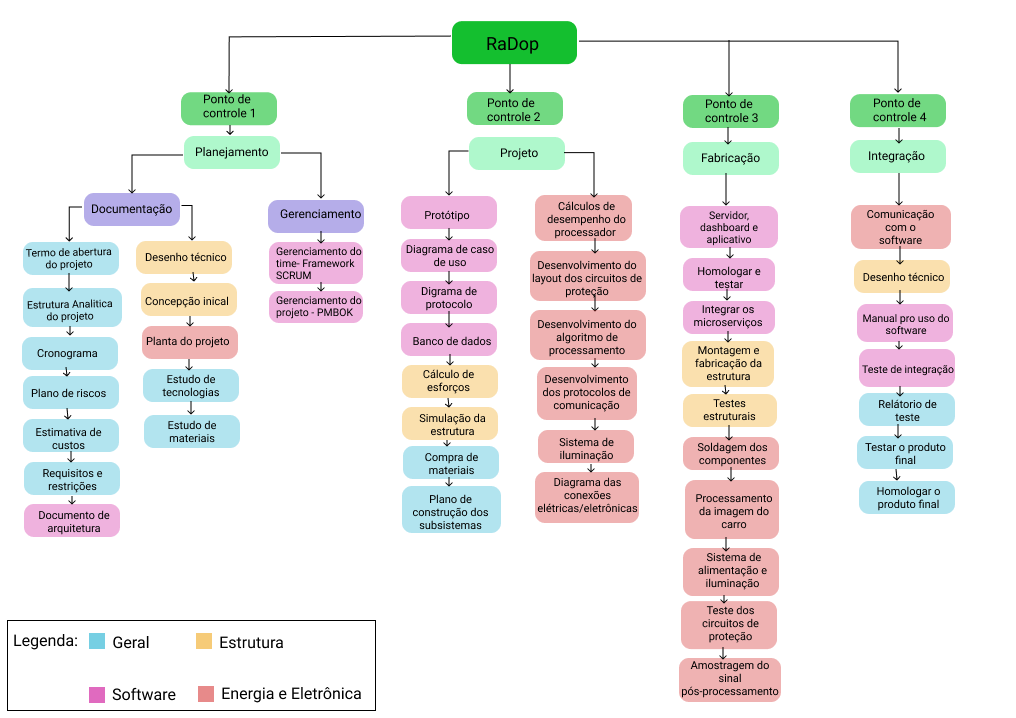
\includegraphics[width=\textwidth]{eap}}
    \caption{\label{fig:eap} EAP do projeto}
\end{figure}
\section{Lista É/Não é}
\subsection{É}

\begin{itemize}
	\item É um radar de efeito \textit{Doppler};
	\item É um detector de veículos;
	\item É composto de sistema capaz de reconhecer placa de carros acima da velocidade da rodovia;
	\item É projetado para pistas simples;
	\item É para ser utilizados em curvas;
	\item É para áreas de região serrana;
	\item É configurado para sinalizar por meio de sinalização luminosa;
	\item É um sistema de prevenção de acidentes;
	\item É composto de sistema energético fotovotaico.
\end{itemize}
\subsection{Não é}

\begin{itemize}
	\item Não é para ser utilizado em pistas duplas;
	\item Não é para usar em trechos de rodovias contínuos;
	\item Não é para utilizar em cruzamentos;
	\item Não é para aplicar multa em carros infratores;
	\item Não é para ser utilizado em sinalização de trânsito;
	\item Não é um sistema de fiscalização de trânsito.
\end{itemize}

\section{Requisitos}
\subsection{Eletrônica}

Os requisitos de eletrônica são:
	
\begin{itemize}
	\item Detectar a aproximação do carro na via;
    \item Calcular a velocidade relativa do carro;
    \item Implementar uma comunicação entre os dois radares para determinar a emissão do alerta;
    \item Criar uma interface entre o radar e o motorista para visualização do alerta;
    \item Capturar imagem traseira do carro com a placa quando este passar acima da velocidade permitida;
    \item Projetar e construir circuitos de proteção para o dispositivos eletrônicos;
    \item Fazer o pré-processamento da imagem para reconhecimento da placa do veículo;
    \item Determinar a velocidade máxima do veículo para melhor captura da placa;
    \item Determinar a distância do veículo em relação ao radar para melhor captura da placa;
    \item Determinar a distância máxima entre os dois radares;
    \item Selecionar e implementar os protocolos de comunicação entre os dois radares;
    \item Selecionar e implementar os protocolos de comunicação entre os radares e o servidor;
     \item Determinar a capacidade de armazenamento mínimo necessário para guardar dados quando a comunicação entre o radar e o servidor estiver fora de serviço;
     \item Determinar a velocidade mínima de transmissão de dados entre os radares para emissão de alerta;
     \item Determinar e implementar a estrutura do pacote de dados a ser enviado para o servidor contendo todas as informações necessárias;
     \item Transmitir para o servidor a velocidade, a imagem da placa pré-processada  e outras informações sobre o funcionamento do sistema.
\end{itemize}    
    
    As restrições de eletrônica são:

\begin{itemize}

	\item Se limitar em apenas reconhecer a placa do veículo, e não gerar a multa;
	\item Falha de comunicação entre os radares e o servidor por no máximo 3 dias;
	\item O veículo deve estar em uma velocidade igual ou menor que a velocidade máxima estabelecida para captura da placa;
	\item A captura da câmera deve ser apenas da traseira do veículo, devido ao fato de motos terem placa apenas na parte de trás, unificando o processo;
	\item A distância máxima entre os radares deve ser de 1 km.
	
\end{itemize} 	
	
\subsection{Energia}
\begin{itemize}
	\item O sistema deve conter painéis fotovoltaicos que promoverão a fonte de alimentação para todos os componentes do sistema;
	\item O sistema deve garantir o máximo aproveitamento energético;
	\item O sistema deve conter circuitos de controle de tensão e corrente;
	\item O sistema deve garantir o funcionamento seguro e contínuo do Radar;
	\item O sistema deve conter um circuito de iluminação para servir de alerta aos motoristas.

\end{itemize}

As restrições de Energia são:
\begin{itemize}
   \item Dependêcia do clima para a geração de energia;
   \item Localização Geografica;
   \item Temperatura média;
   \item Índices de radiação solar;
   \item Posicionamento das placas em relação a radiação solar;
   \item Horário de exposição;
   \item Existência de sombramento.
 \end{itemize}
\subsection{Estrutura}

Os requisitos de Estruturas são:

\begin{itemize}
	\item A estrutura deve suportar o peso de todos os componentes com margem de segurança para eventuais cargas não estimadas;
	\item Deve possuir resistência a ação climática, especificamente a radiação solar, temperatura elevada e corrosão devido a exposição a chuva;
	\item A placa solar que fornecerá a energia do sistema deverá ficar na parte superior do conjunto, a estrutura deve ser pensada e dimensionada com isso em mente;
	\item Os sistemas de antena e câmera deverão estar em montantes articulados para que a incidência possa ser ajustada;
	\item A estrutura deve conter suporte para manutenção facilitada, permitindo o acesso aos componentes de maneira facilitada;
	\item O vento incidente devido a região de instalação deve também ser suportado pela estrutura;
\end{itemize}

As restrições de Estruturas são:

\begin{itemize}
	\item Os materiais não podem ser suscetíveis a corrosão, a ruptura por radiação e temperatura solar e não podem comprometer o funcionamento dos sistemas eletrônicos;
	\item A estrutura não pode ter área de contato com o vento muito elevado;
	\item Os compartimentos de instalação dos eletrônicos não pode possuir entrada para água ou detritos externos;
	\item Os compartimentos não podem estar totalmente isolados, permitindo acesso para reparos e manutenção;
	\item Os materiais selecionados não podem impedir o funcionamento de qualquer um dos componentes eletrônicos, a exemplo de impedir a emissão ou recepção do radar.
\end{itemize}

\subsection{Software}

Os requisistos de \emph{software} são:

\begin{itemize}
    \item Interface do \emph{Dashboard};
    \item Interface do aplicativo;
    \item Manual de uso dos \emph{softwares} : microsserviços, aplicativo e \emph{Dashboard}.;
    \item Funcionar com conexão a redes (\emph{internet});
    \item Ser capaz de lidar e recuperar de falhas e erros como: conexão, processamento, entre outros;
    \item \emph{Software} devem ser manuteníveis e evolutíveis;
    \item Os \emph{software} devem ser testáveis e testados;
    \item O \emph{Software} deve mostrar dados e informações do Radar;
    \item O \emph{Software} deve ser capaz de tomar decisões para alertar socorristas a respeito de prováveis acidentes automobilísticos;
    \item O \emph{Software} deve ser capaz de tomar decisões para alertar usuários de possíveis situações de risco;
    \item O \emph{Software} deve ser capaz de mostrar informações gerenciais com os dados do Radar.
\end{itemize}

As restrições de \emph{software} são:

\begin{itemize}
    \item O emph{software} necessita estar sempre conectado à internet para comunicação e, consequentemente, para o correto funcionamento;
    \item O aplicativo de manutenção irá auxiliar apenas com o essencial;
    \item O aplicativo só funcionará em aparelhos \emph{Android};
    \item A linguagem de cada microsserviço (assim como \emph{framework}/tecnologia) será definida dada necessidade (performance, armazemanento e etc) dos mesmos;
\end{itemize}

\section{\emph{Stakeholders}}

\subsection {Cliente}

Governo Federal ou Estadual no âmbito de melhorar a segurança nas estradas, diminuindo o número de acidentes acidentes. 

\subsection {Docentes}

Professores da Universidade de Brasília (UnB) que ministram a disciplina Projeto Integrador 2 que tem como papel orientar e avaliar o desenvolvimento do projeto até o produto final.

\section{Recurso humanos}

 De modo a ter uma melhor organização, a equipe foi dividida em subgrupos, onde cada subgrupo tem um gerente técnico, além disso a equipe também conta com um gerente de qualidade e um coordenador geral. Na Fig. \ref{fig:organograma} mostra o organograma da equipe e o nome de cada integrante por função.
 
\begin{figure}[h]
\centering
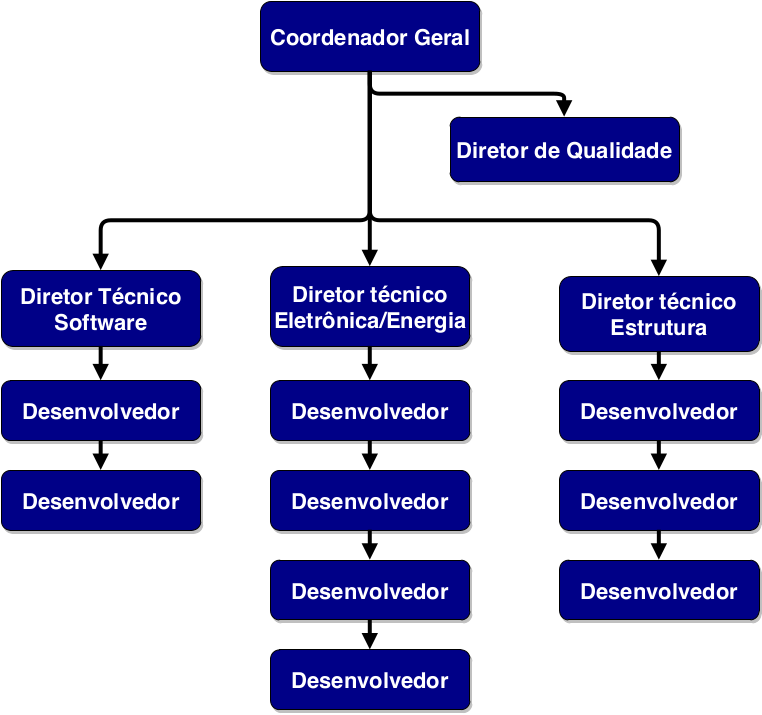
\includegraphics[scale = 0.5]{organograma}
\caption{Organograma}\label{fig:organograma}
\end{figure} 

A seguir estão os nomes de cada integrante separado por área:

\begin{itemize}
\item Eletrônica e Energia

-Brenda Bianca Neves Dias\\
-Danyelle Bemfica da Rocha\\
-\textbf{Elpidio Cândido de Araújo Bisneto -> Coordenador geral}\\
-Filipe de Souza Freitas\\
-\textbf{Kewin Kuster -> Diretor técnico}\\
-Rodrigo Sousa Santos

\item Estrutura

-\textbf{Daniele Dias Sousa -> Diretora de qualidade}\\
-Fernanda Resende Muro Martinez\\
-Luiz Felipe Martins Cruz\\
-Pedro Henrique Nazareno Halabi\\
-\textbf{Rafael Mascarenhas dos Santos -> Diretor técnico}

\item Software

-Diego Barbosa da Mota França\\
-\textbf{João Pedro Sconetto -> Diretor técnico}\\
-Mariana de Souza Mendes 


\end{itemize}

\subsection{Ferramentas de gerenciamento}

Foram selecionadas algumas ferramentas de gerenciamento, afim de organizar o trabalho da equipe.

\emph{\textbf{Discord:}} É um aplicativo de comunicação onde a equipe pode se comunicar de forma rápida com mensagens, além disso permite o envio de vídeos, imagens e documentos. Outra vantagem da ferramenta é a possibilidade de fazer áudio-conferência com mais de 10 pessoas.

\emph{\textbf{Google drive:}} Ferramenta em nuvem para armazenamento e compartilhamento de arquivos.

\emph{\textbf{GitHub e Texmaker:}} \emph{Texmaker} é uma ferramenta para edição de texto em \emph{Latex} e o \emph{GitHub} é um ferramenta de desenvolvimento.

\emph{\textbf{Trello:}} O Trello é bastante conhecido por ser uma ferramenta de gerenciamento de projetos. 

\section{Cronograma de atividades}

Para uma melhor visualização, o leitor será redirecionado para o local de hospedagem do \href{https://docs.google.com/spreadsheets/d/1dcQycQPI0zbYMb-VP8nqHmpS_v0IhSz5-u9oQcoDKUI/edit?usp=sharing}{cronograma de atividades}.

\section{Milestones Identificados}

A Tabela \ref{tab:milestones} apresenta as datas de entregáveis.

\begin{table}[h]
\caption{Milestones}
\label{tab:milestones}
\begin{tabular}{|c|c|}
\hline
\rowcolor[HTML]{9B9B9B} 
\textbf{Atividades}                                                                                                    & \textbf{Data de entrega}                               \\ \hline
Entrega de relatório do Ponto de Controle 1                                                                            & 03/04/2019                                   \\ \hline
Ponto de Controle 1 (PC1)                                                                                              & \multicolumn{1}{l|}{05/04/2019 a 12/04/2019} \\ \hline
Entrega de relatório do Ponto de Controle 2                                                                            & 03/05/2019                                   \\ \hline
Ponto de Controle 2 (PC2)                                                                                              & 08/05/2019 a 15/05/2019                      \\ \hline
Prova 1 (P1)                                                                                                           & 31/05/2019                                   \\ \hline
Entrega de relatório do Ponto de Controle 3                                                                            & 05/06/2019                                   \\ \hline
Ponto de Controle 3 (PC3)                                                                                              & 07/06/2019 a 14/07/2019                      \\ \hline
Ponto de Controle 4 (PC4)                                                                                              & 01/07/2019 a 05/07/2019                      \\ \hline
Data de reapresentação do PC4                                                                                          & 08/07/2019                                   \\ \hline
Entrega de relatório do Ponto de Controle 4                                                                            & 10/07/2019                                   \\ \hline
\begin{tabular}[c]{@{}c@{}}Apresentação de projetos na FIT/FGA (Feira de Inovação\\  e Tecnologia da FGA)\end{tabular} & 10/07/2019                                   \\ \hline
\end{tabular}
\end{table}

\section{Estimativa de custos}

\subsection{Engenharia de Software}

A Tabela \ref{tab:custos_software} apresenta todos os gastos que serão necessários para a equipe de software, assim como todas as aquisições que serão feitas durante o projeto:

\begin{table}[h]
	\caption{Estimativa de custos de \emph{software}}
	\label{tab:custos_software}
    \resizebox{\textwidth}{!}{\begin{tabular}{|c|c|c|c|c|c|c|}
    \hline
    \textbf{Nome do produto} & \textbf{Descrição}                      & \textbf{Marca} & \textbf{Preço unitário} & \textbf{Quantidade} & \textbf{Fornecedor} & \textbf{Orçamento} \\ \hline
    Servidor                 & Máquina para execução dos serviços      & ---            & US\$ 10,00 por mês      & 5 meses             & Digital Ocean       & US\$ 50,00         \\ \hline
    Raspberry Pi 3 B         & Placa de IoT para execução de softwares & Raspberry      & R\$ 279,90              & 1 unidade           & FilipeFlop          & R\$ 279,90         \\ \hline
    \end{tabular}}
\end{table}

OBS: Essa planilha poderá ser atualizado dependendo de necessidades que surgirem durante a execução do projeto.


\subsection{Engenharia Eletrônica}

A Tabela \ref{custos_eletronica} apresenta a estimativa de custos gerais, assim como os insumos já adquiridos.

\begin{table}[h]
\centering
\caption{Estimativa de custos de eletrônica}
\label{custos_eletronica}
\begin{tabular}{|c|c|c|c|c|}
\hline
\multicolumn{5}{|c|}{Eletrônica} \\ \hline
Quantidade & Material & Valor Unitário & Total & Fornecedor \\ \hline
02 & BeagleBone & R\$ 320,00 & R\$ 640,00 & Mercado Livre \\ \hline
02 & Módulos GSM & R\$ 99,90 & R\$ 199,90 & TDTEC \\ \hline
02 & Módulos RF & R\$ 32,90 & R\$ 65,80 & HU Infinito \\ \hline
10 & \begin{tabular}[c]{@{}c@{}}Componentes para Placa\\  de Circuito Impresso\end{tabular} & R\$ 40,00 & R\$ 400,00 & HU Infinito \\ \hline
02 & Antena painel & R\$ 108,80 & R\$ 217,60 & Emprestado \\ \hline
02 & BladeRF NUAND & R\$ 3.000,00 & R\$ 6.000,00 & Emprestado \\ \hline
02 & Circulador & R\$ 150,00 & R\$ 300,00 & Emprestado \\ \hline
02 & Câmera & R\$ 1.000,00 & R\$ 2.000,00 & Em análise \\ \hline
X & Componentes diversos & R\$ 50,00 & R\$ 50,00 & HU Infinito \\ \hline
Total & - - & - - & R\$ 9873,30 & - - \\ \hline
\end{tabular}
\end{table}
\pagebreak
\subsection{Engenharia de Energia}

A Tabela \ref{tab:custos_energia} apresenta os gastos preliminares de energia, assim como todas as aquisições que serão feitas durante o projeto:

\begin{table}[h]
\caption{Estimativa de custos de energia}
\label{tab:custos_energia}
\begin{tabular}{|c|c|c|c|c|}
\hline
\multicolumn{5}{|c|}{Energia}                                                 \\ \hline
Material             & Preço         & Quantidade & Total         & Marca     \\ \hline
Painel Fotovoltaico  & R\$ 420,00  & 2          & R\$ 840,00  & Komaes    \\ \hline
Bateria              & R\$ 300,00  & 2          & R\$ 600,00  & Unipower  \\ \hline
Controlador de Carga & R\$ 65,00  & 2          & R\$ 130,00  & Automad3D \\ \hline
Painel de LED        & R\$ 23,00  & 2          & R\$ 46,00 & Briwax    \\ \hline
Lâmpada de LED       & R\$ 38,00 & 2          & R\$ 76,00 & PXT         \\ \hline
\end{tabular}
\end{table}

\section{Viabilidades financeira}

O projeto será executado atendendo os requisitos apresentados, acima foram listados todos os insumos que serão necessários para a realização. Alguns insumos foram fornecidos pelos professores da matéria ou outros professores ou os membros do grupo já tinham. A Tabela \ref{tab:elps1} mostra o valor estimado total do projeto. 

% Please add the following required packages to your document preamble:
% \usepackage[table,xcdraw]{xcolor}
% If you use beamer only pass "xcolor=table" option, i.e. \documentclass[xcolor=table]{beamer}
\begin{table}[h]
\centering
\caption{Valor estimado dos insumos totais}
\label{tab:elps1}
\begin{tabular}{|c|c|c|c|c|l|}
\hline
Área                                                          & Eletrônica                                               & Energia                                               & Estrutura                                      & Software                                                & Total                                \\ \hline
Custos totais (R\$)                                           & \cellcolor[HTML]{34CDF9}R\$ 9873,30                      & \cellcolor[HTML]{FCFF2F}R\$ 1692                      & \cellcolor[HTML]{9B9B9B}-                      & \cellcolor[HTML]{34FF34}R\$ 472,92                      & \cellcolor[HTML]{FD6864}R\$ 12037,92 \\ \hline
\begin{tabular}[c]{@{}c@{}}Custos com os insumos\\ disponíveis (R$\$$)\end{tabular} & \multicolumn{1}{l|}{\cellcolor[HTML]{34CDF9}R\$ 3253,30} & \multicolumn{1}{l|}{\cellcolor[HTML]{FFFE65}R\$ 1692} & \cellcolor[HTML]{9B9B9B}-                      & \multicolumn{1}{l|}{\cellcolor[HTML]{34FF34}R\$ 192,72} & \cellcolor[HTML]{FD6864}R\$5138,02   \\ \hline
\end{tabular}
\end{table}

A Tabela \ref{tab: elps2} mostra o valor estimado sem o valor dos insumos que o grupo já tem.

\begin{table}[h]
\centering
\caption{Valor dos insumos já adquiridos}
\label{tab: elps2}
\begin{tabular}{|c|c|}
\hline
                              & Cliente Real \\ \hline
Pessoas na equipe             & 14           \\ \hline
Duração do projeto (em meses) & 3            \\ \hline
Valor total (R\$)             & R\$ 5138,02  \\ \hline
Valor por pessoa (R\$)        & R\$ 367      \\ \hline
Contribuição mensal (R\$)     & R\$ 122,33   \\ \hline
\end{tabular}
\end{table}

\section{Levantamento de riscos}
\subsection{Geral}

\begin{itemize}
    \item RGN 1 - Saída de um membro da equipe;
    \item RGN 2 - Desentendimentos entre membros da equipe;
    \item RGN 3 - Membro da equipe temporariamente impossibilitado de trabalhar;
    \item RGN 4 - Mudança do escopo do projeto;
    \item RGN 5 - Equipe com dificuldades no uso das tecnologias usadas no projeto;
    \item RGN 6 - Dívida técnica por não conseguir entregar as histórias previstas;
    \item RGN 7 - Membros com carga excessiva de trabalho;
    \item RGN 8 - Atraso no roadmap do projeto.
\end{itemize}

\subsection{\emph{Software}}
\begin{itemize}
    \item RSN 1 - Falta de infraestrutura para o desenvolvimento do \emph{software} (configuração de ambiente de desenvolvimento, configuração do \emph{github}, etc);
    \item RSN 2 - Descontinuação de pacotes de dependências usados;
    \item RSN 3 - Dificuldades para realizar o \emph{deploy};
    \item RSN 4 - Atraso na implementação da arquitetura do projeto;
    \item RSN 5 - Dificuldades com as tecnologias relacionadas à microsserviços;
    \item RSN 6 - Problemas na comunicação entre os \emph{softwares} e o radar.
\end{itemize}

\subsection{Energia}
\begin{itemize}
   \item RSN 1 - Alimentação insuficiente ao Radar;
   \item RSN 2 - Curta vida útil dos equipamentos; 
   \item RSN 3 - Queima dos componentes elétricos;
   \item RSN 4 - Tamanho da bitola dos cabos insuficiente para a quantidade de tensão e corrente;
   \item RSN 5 - Montagem mal feita;
   \item RSN 6 - Altura da fonte de alimentação segura para realizar manutenção e instalação;
   \item RSN 7 - Pista movimentada no dia da instalação;
   \item RSN 8 - Negligenciamento da dissipação de calor;
   \item RSN 9 - Estrutura mal dimensionada para o suporte e proteção do sistema de alimentação.
\end{itemize}

\subsection{Eletrônica}

\begin{itemize}

	\item RSN 1 - Veículos muito próximos;
	\item RSN 2 - Veículo acima da velocidade máxima de captura da câmera;
	\item RSN 3 - Queda de energia do sistema;
	\item RSN 4 - Falha na comunicação entre os radares e/ou entre os radares e o servidor;
	\item RSN 5 - Interferência entre os sinais do radar e do módulo de comunicação entre os radares;
	\item RSN 6 - Captura da câmera com qualidade inferior ao necessário para processamento da imagem;
	
\end{itemize} 	

\subsection{Estruturas}
\begin{itemize}
	\item RSN 1 - Atrasos por fornecimento de materiais;
	\item RSN 2 - Aterramento mal feito podendo causar a corrosão da estrutura ou sua fundação;
	\item RSN 3 - Montagem mal feita;
	\item RSN 4 - Interferência da estrutura com os equipamentos de radiofrequência;
	\item RSN 5 - Atrasos causados por problemas de simulações e modelagem;
	\item RSN 6 - Curto circuito de componentes eletrônicos causados pela estrutura;
\end{itemize}
